% !TEX root = ../../main.tex


\begin{figure}[!htb]
\centering
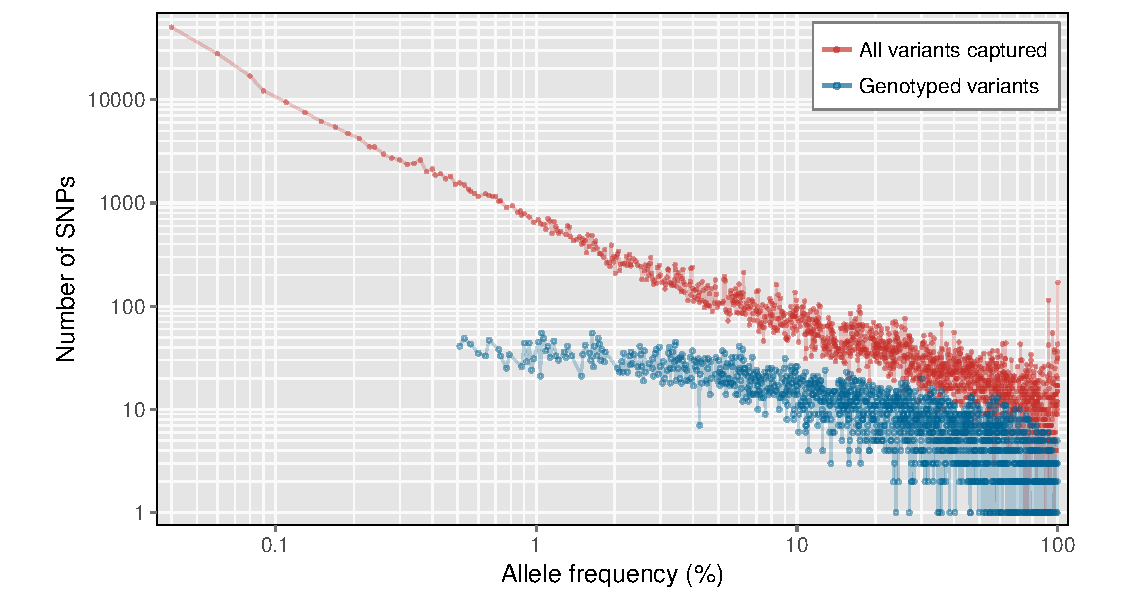
\includegraphics[width=0.9\textwidth]{./img/ch2/sfs_got2d}
\Caption{Site frequency spectrum of variants captured in GoT2D (chromosome 20)}
{The \glsentryfull{sfs} is shown for SNPs as captured in the full \gls{got2d} dataset (\emph{red}) and SNPs genotyped using \emph{Illumina Omni2.5 Array} (\emph{blue}), given the allele frequencies observed in the full \gls{got2d} sample for chromosome~20, after removing singletons and monomorphic sites.}
{fig:sfs_got2d}
\end{figure}
